\documentclass[11pt,]{article}
\usepackage[left=1in,top=1in,right=1in,bottom=1in]{geometry}
\newcommand*{\authorfont}{\fontfamily{phv}\selectfont}
\usepackage[]{mathpazo}


  \usepackage[T1]{fontenc}
  \usepackage[utf8]{inputenc}



\usepackage{abstract}
\renewcommand{\abstractname}{}    % clear the title
\renewcommand{\absnamepos}{empty} % originally center

\renewenvironment{abstract}
 {{%
    \setlength{\leftmargin}{0mm}
    \setlength{\rightmargin}{\leftmargin}%
  }%
  \relax}
 {\endlist}

\makeatletter
\def\@maketitle{%
  \newpage
%  \null
%  \vskip 2em%
%  \begin{center}%
  \let \footnote \thanks
    {\fontsize{18}{20}\selectfont\raggedright  \setlength{\parindent}{0pt} \@title \par}%
}
%\fi
\makeatother




\setcounter{secnumdepth}{3}

\usepackage{longtable,booktabs}

\usepackage{graphicx,grffile}
\makeatletter
\def\maxwidth{\ifdim\Gin@nat@width>\linewidth\linewidth\else\Gin@nat@width\fi}
\def\maxheight{\ifdim\Gin@nat@height>\textheight\textheight\else\Gin@nat@height\fi}
\makeatother
% Scale images if necessary, so that they will not overflow the page
% margins by default, and it is still possible to overwrite the defaults
% using explicit options in \includegraphics[width, height, ...]{}
\setkeys{Gin}{width=\maxwidth,height=\maxheight,keepaspectratio}

\title{Ecología numérica de la familia Myrtaceae en la parcela permanente de
50-ha en Barro Colorado, lago Gatún, Panamá\\
Subtítulo\\
Subtítulo  }



\author{\Large Rosee Aurelina Féliz Méndez\vspace{0.05in} \newline\normalsize\emph{Estudiante, Universidad Autónoma de Santo Domingo (UASD)}  }


\date{}

\usepackage{titlesec}

\titleformat*{\section}{\normalsize\bfseries}
\titleformat*{\subsection}{\normalsize\itshape}
\titleformat*{\subsubsection}{\normalsize\itshape}
\titleformat*{\paragraph}{\normalsize\itshape}
\titleformat*{\subparagraph}{\normalsize\itshape}

\titlespacing{\section}
{0pt}{36pt}{0pt}
\titlespacing{\subsection}
{0pt}{36pt}{0pt}
\titlespacing{\subsubsection}
{0pt}{36pt}{0pt}





\newtheorem{hypothesis}{Hypothesis}
\usepackage{setspace}

\makeatletter
\@ifpackageloaded{hyperref}{}{%
\ifxetex
  \PassOptionsToPackage{hyphens}{url}\usepackage[setpagesize=false, % page size defined by xetex
              unicode=false, % unicode breaks when used with xetex
              xetex]{hyperref}
\else
  \PassOptionsToPackage{hyphens}{url}\usepackage[unicode=true]{hyperref}
\fi
}

\@ifpackageloaded{color}{
    \PassOptionsToPackage{usenames,dvipsnames}{color}
}{%
    \usepackage[usenames,dvipsnames]{color}
}
\makeatother
\hypersetup{breaklinks=true,
            bookmarks=true,
            pdfauthor={Rosee Aurelina Féliz Méndez (Estudiante, Universidad Autónoma de Santo Domingo (UASD))},
             pdfkeywords = {Myrtaceae, Ecología numérica, BCI},  
            pdftitle={Ecología numérica de la familia Myrtaceae en la parcela permanente de
50-ha en Barro Colorado, lago Gatún, Panamá\\
Subtítulo\\
Subtítulo},
            colorlinks=true,
            citecolor=blue,
            urlcolor=blue,
            linkcolor=magenta,
            pdfborder={0 0 0}}
\urlstyle{same}  % don't use monospace font for urls

% set default figure placement to htbp
\makeatletter
\def\fps@figure{htbp}
\makeatother

\usepackage{pdflscape} \newcommand{\blandscape}{\begin{landscape}}
\newcommand{\elandscape}{\end{landscape}}


% add tightlist ----------
\providecommand{\tightlist}{%
\setlength{\itemsep}{0pt}\setlength{\parskip}{0pt}}

\begin{document}
	
% \pagenumbering{arabic}% resets `page` counter to 1 
%
% \maketitle

{% \usefont{T1}{pnc}{m}{n}
\setlength{\parindent}{0pt}
\thispagestyle{plain}
{\fontsize{18}{20}\selectfont\raggedright 
\maketitle  % title \par  

}

{
   \vskip 13.5pt\relax \normalsize\fontsize{11}{12} 
\textbf{\authorfont Rosee Aurelina Féliz Méndez} \hskip 15pt \emph{\small Estudiante, Universidad Autónoma de Santo Domingo (UASD)}   

}

}








\begin{abstract}

    \hbox{\vrule height .2pt width 39.14pc}

    \vskip 8.5pt % \small 

\noindent Resumen del manuscrito


\vskip 8.5pt \noindent \emph{Keywords}: Myrtaceae, Ecología numérica, BCI \par

    \hbox{\vrule height .2pt width 39.14pc}



\end{abstract}


\vskip 6.5pt


\noindent  \section{Introducción}\label{introducciuxf3n}

La isla de Barro Colorado (BCI, por sus siglas en inglés) se formó al
término del canal de Panamá en 1974, desde su creación se ha utilizado
como centro de investigación debido a su gran reserva natural. Se
considera monumento natural protegido por el gobierno de Panamá junto a
las penínsulas Peña Blanca, Bohío, Buena Vista, Frijoles y Gigante. La
parcela permanente de 50 hectáreas se encuentra en el bosque húmedo
tropical de la isla de Barro Colorado. Se estableció en 1980, desde
entonces se han realizado 8 censos (aprox. 1 cada 5 años) en cual se
toman en cuenta árboles de tallos leñosos con un diámetro a la altura
del pecho (DAP) mayor a 10 mm, y como resultado en cada censo, se han
identificado, censado y mapeado más de 350, 000 árboles
individuales(Hubbell, Condit, \& Foster, 2021).

Se ha seleccionado el censo número 8 de esta reserva natural por ser el
más reciente y a esta reserva natural en particular debido a la gran
cantidad disponible de datos censales que a través de la Ecología
numérica nos permitirán conocer rasgos básicos de la estructura y
composición de la comunidad de plantas mirtáceas en relación con
factores ambientales.

Las mirtáceas ( Myrtaceae Juss) son una familia de plantas leñosas del
orden Myrtales. La mayoría de las especies son árboles, también hay
muchas que son arbustos o subarbustos. Algunas especies producen flores
y frutos, otras raíces adventicias. Se distribuyen principalmente en
zonas tropicales y templadas, con poca representación en la región
africana. La familia cuenta con unos 142 géneros y más de 5.500
especies, incluyendo \emph{Psiloxylon} y \emph{Heteropyxis}, también
pueden ser citadas por otros autores como familias monogenéricas
Psiloxylaceae y Heteropyxidaceae. Cabe destacar que la familia integra
los árboles más altos (110-140 m) del planeta ( \emph{Eucalyptus}) y al
género más numeroso (1200‒1800 especies) que existe ( \emph{Syzygium}),
los subarbustos rizomatosos de los géneros de la sabana (
\emph{Psidium}, \emph{Campomanesia} y \emph{Eugenia}), el género
\emph{Metrosideros} que contiene especies arbóreas con muchas raíces
adventicias, y otros géneros son lianas trepadoras de raíces. También
hay un mangle, el monotípico \emph{Osbornia}, un pequeño árbol que
carece de neumatóforos (Wilson, 2010).

R

En este trabajo se harán estudios de asociación, agrupamiento,
diversidad y ecología espacial en relación a factores ambientales con
los datos disponibles del censo número de 8 de la parcela permanente de
50-ha con ecología numérica en R para comprender mejor la estructura y
composición de la comunidad de mirtáceas en la foresta tropical de Barro
Colorado.

\section{Metodología}\label{metodologuxeda}

Ambito geográfico

La parcela permanente de 50 hectáreas es un bosque húmedo tropical que
fue establecido en 1980 por Stephen Hubbell y Robin Foster en la meseta
central de la isla de Barro Colorado (latitud 9\(^\circ\)~9'N, longitud
79\(^\circ\)~50'O). Posee 1,000 m de largo por 500 m de ancho, se divide
en 1250 cuadrantes de 20x20 m (ver figura \ref{fig:mapa_cuadros_bci}).
En la parcela, todos los tallos leñosos con un DAP mayor o igual a 1 cm
se encuentran marcados, enumerados, mapeados e identicados hasta el
nivel de especie. Cada 5 años, esta parcela es censada para evaluar el
cremiento, la mortalidad y el reclutamiento de nuevas generaciones de
plantas. Como resultado de estos censos se han registrado mas de 300
especies de árboles, arbustos y palmas con el próposito de conocer la
historia de vida de las especies, interacciones y dinámica de la
comunidad (Pérez et al., 2005).

\begin{figure}
\centering
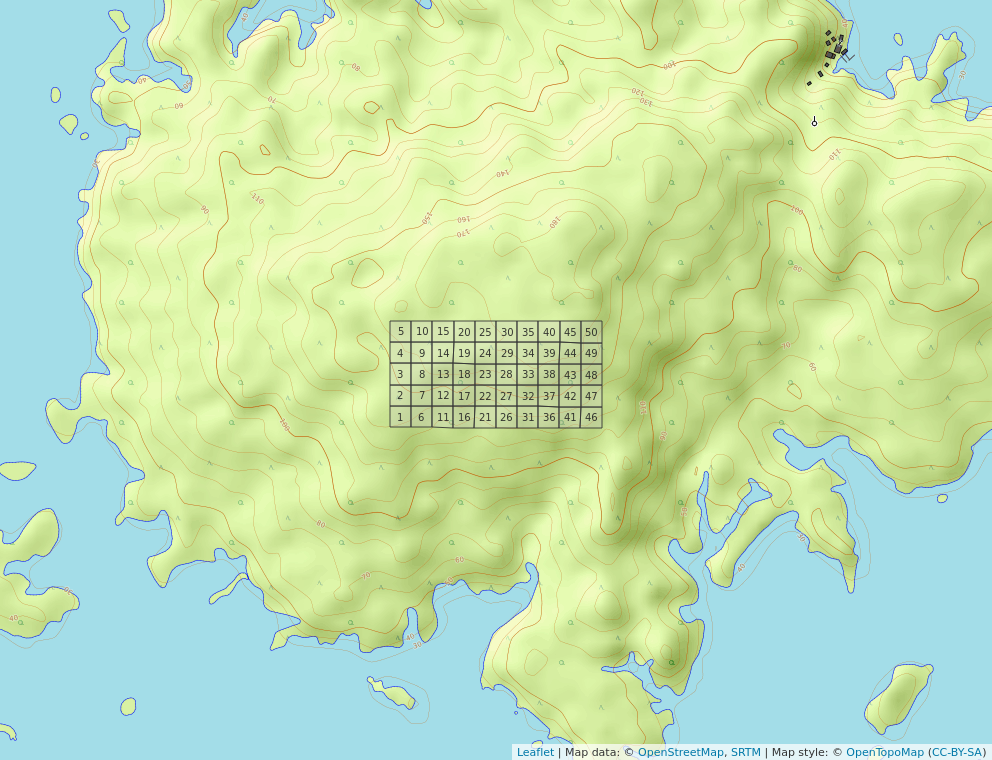
\includegraphics[width=0.50000\textwidth]{mapa_cuadros.png}
\caption{Parcela permanente de 50-ha dela isla Barro Colorado, lago
Gatún, Panamá \label{fig:mapa_cuadros_bci}}
\end{figure}

Materiales y Métodos

Se exploraron los datos del censo número 8 disponibles en la página web
del censo (Hubbell et al., 2021), organizados en dos matrices: la matriz
de comunidad, la cual recopila la información referente a las especies
de la parcela permanente de 50-ha, y la matriz ambiental, que contiene
la información referente a las variables de suelo, geomorfológicas,
litológicas y de tipo de habitat. Los análisis, tablas, figuras y
gráficos se realizaron con los scripts de análisis de José R. Martínez
(Batlle, 2020) y con ayuda de los paquetes de R para análisis
estadísticos y ecológicos (R Core Team, 2019), cabe destacar los
paquetes \texttt{vegan} (Oksanen et al., 2019), \texttt{tidyverse}
(Wickham, 2017), \texttt{sf} (Pebesma, 2018), \texttt{mapview}
(Appelhans, Detsch, Reudenbach, \& Woellauer, 2019) y \texttt{leaflet}
(Cheng, Karambelkar, \& Xie, 2018) que fueron los más utilizados.

\section{Resultados}\label{resultados}

La familia Myrtaceae está presente en la parcela permanente de 50-ha de
BCI con una abundancia de 5,579 individuos pertenecientes a 7 especies,
de las cuales las más abundantes son \emph{Eugenia galalonensis} y
\emph{Eugenia oerstediana}, representadas con 1,975 y 1,838 individuos
cada una, y las especies más raras son \emph{Psidium
friedrichsthalianum} y \emph{Myrcia gatunensis}, con 58 y 56 individuos
respectivamente (ver tabla \ref{tab:abun_sp}).

\begin{longtable}[]{@{}lr@{}}
\caption{\label{tab:abun_sp}Abundancia por especie de la familia
Myrtaceae}\tabularnewline
\toprule
Latin & n\tabularnewline
\midrule
\endfirsthead
\toprule
Latin & n\tabularnewline
\midrule
\endhead
Eugenia galalonensis & 1975\tabularnewline
Eugenia oerstediana & 1838\tabularnewline
Eugenia coloradoensis & 609\tabularnewline
Chamguava schippii & 541\tabularnewline
Eugenia nesiotica & 502\tabularnewline
Psidium friedrichsthalianum & 58\tabularnewline
Myrcia gatunensis & 56\tabularnewline
\bottomrule
\end{longtable}

\begin{figure}
\centering
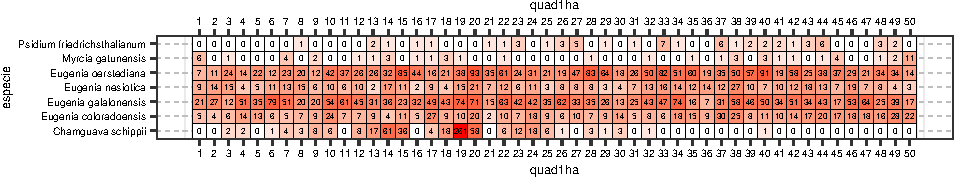
\includegraphics{manuscrito_files/figure-latex/unnamed-chunk-3-1.pdf}
\caption{\label{fig:abun_sp_q}Abundancia de especies por quadrat}
\end{figure}

La distancia de chi-cuadradado y la distancia de Jacard infieren que las
especies del genéro \emph{Eugenia} presentan un patrón de dependencia
(\emph{E. oerstediana}, \emph{E. galalonensis}, \emph{E. nesiotica} y
\emph{E. coloradoensis}), debido a que tienen distancias euclideas muy
pequeñas, es decir, altos grados de asociación; y las especies
\emph{Psidium friedrichsthalianum}, \emph{Myrcia gatunensis} y
\emph{Changuava schippii} presentan un posible patrón independiente, no
parecen asociarse con otras (ver \ref{fig:matriz_Jacard}). El índice de
correlación de Pearson y de Spearman infieren que estos patrones pueden
estar produciéndose debido a la disponibilidad de Al, P y escasez de Ca,
y a la presencia de los atributos del terreno geomorfología de llanura,
elevación media y a una relación negativa con la heterogeneidad
ambiental, geomorfología de vertiente, geomorfología de vaguada y
pendiente media (ver correlogramas \ref{fig:matriz_pearson} y
\ref{fig:matriz_spearman}).

\begin{figure}
\centering
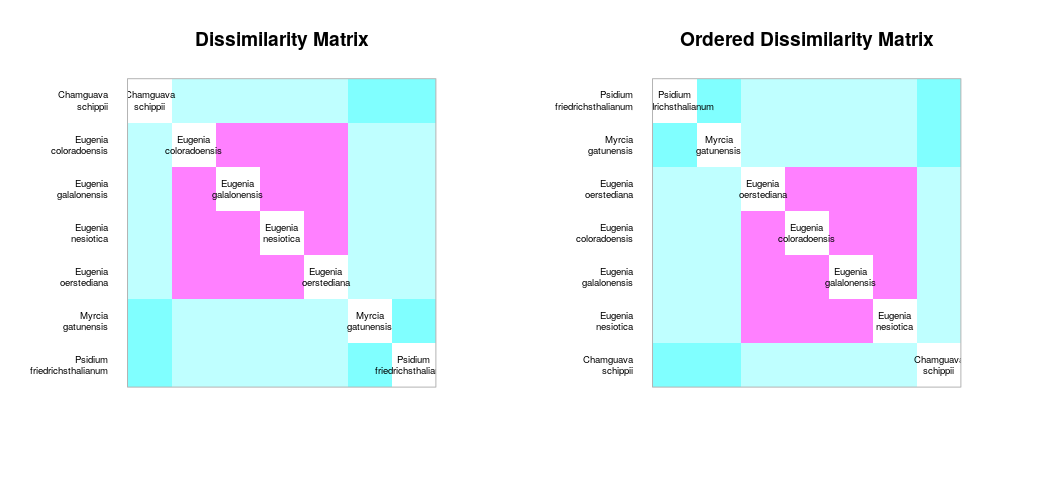
\includegraphics{Disimilaridad_.png}
\caption{Matriz de disimilaridad de Jacard \label{fig:matriz_Jacard}}
\end{figure}

\begin{figure}
\centering
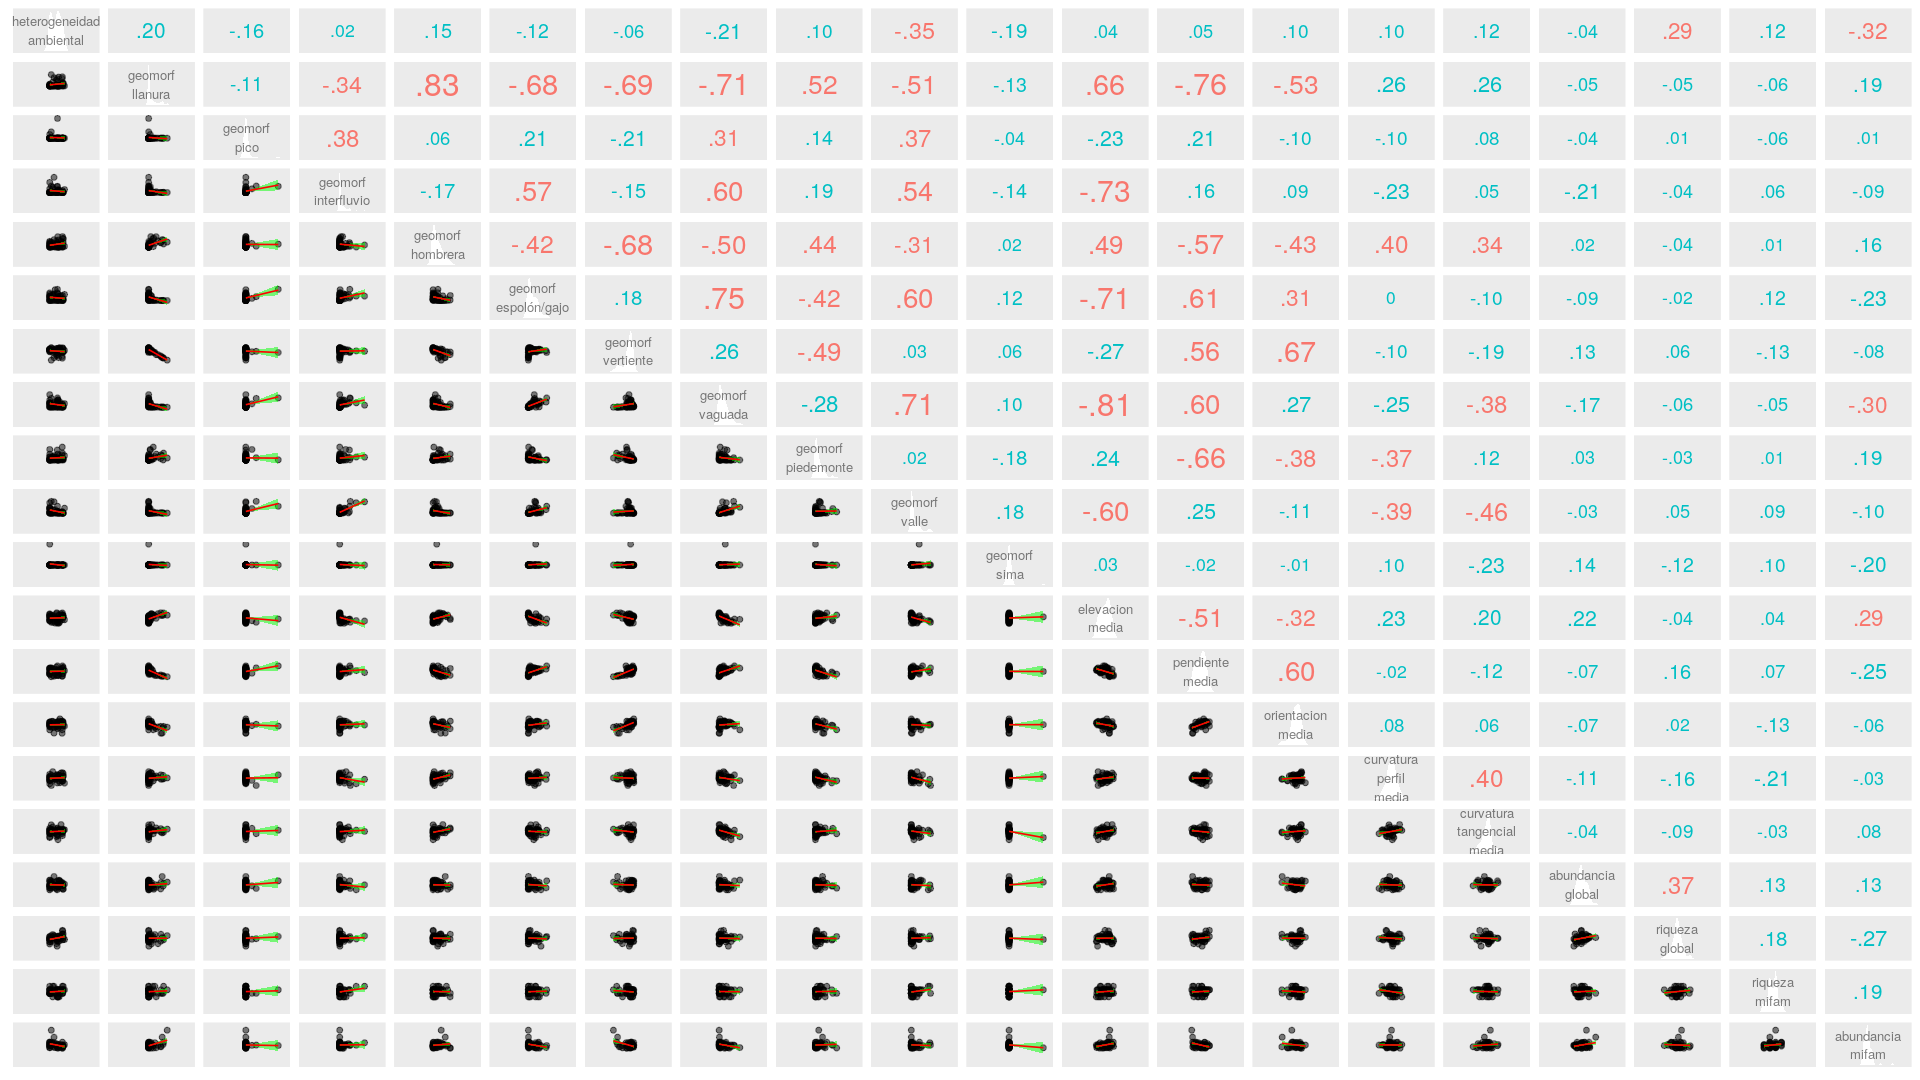
\includegraphics{matriz_correlacion_geomorf_abun_riq_spearman.png}
\caption{Matriz de correlación, índice Pearson
\label{fig:matriz_pearson}}
\end{figure}

\begin{figure}
\centering
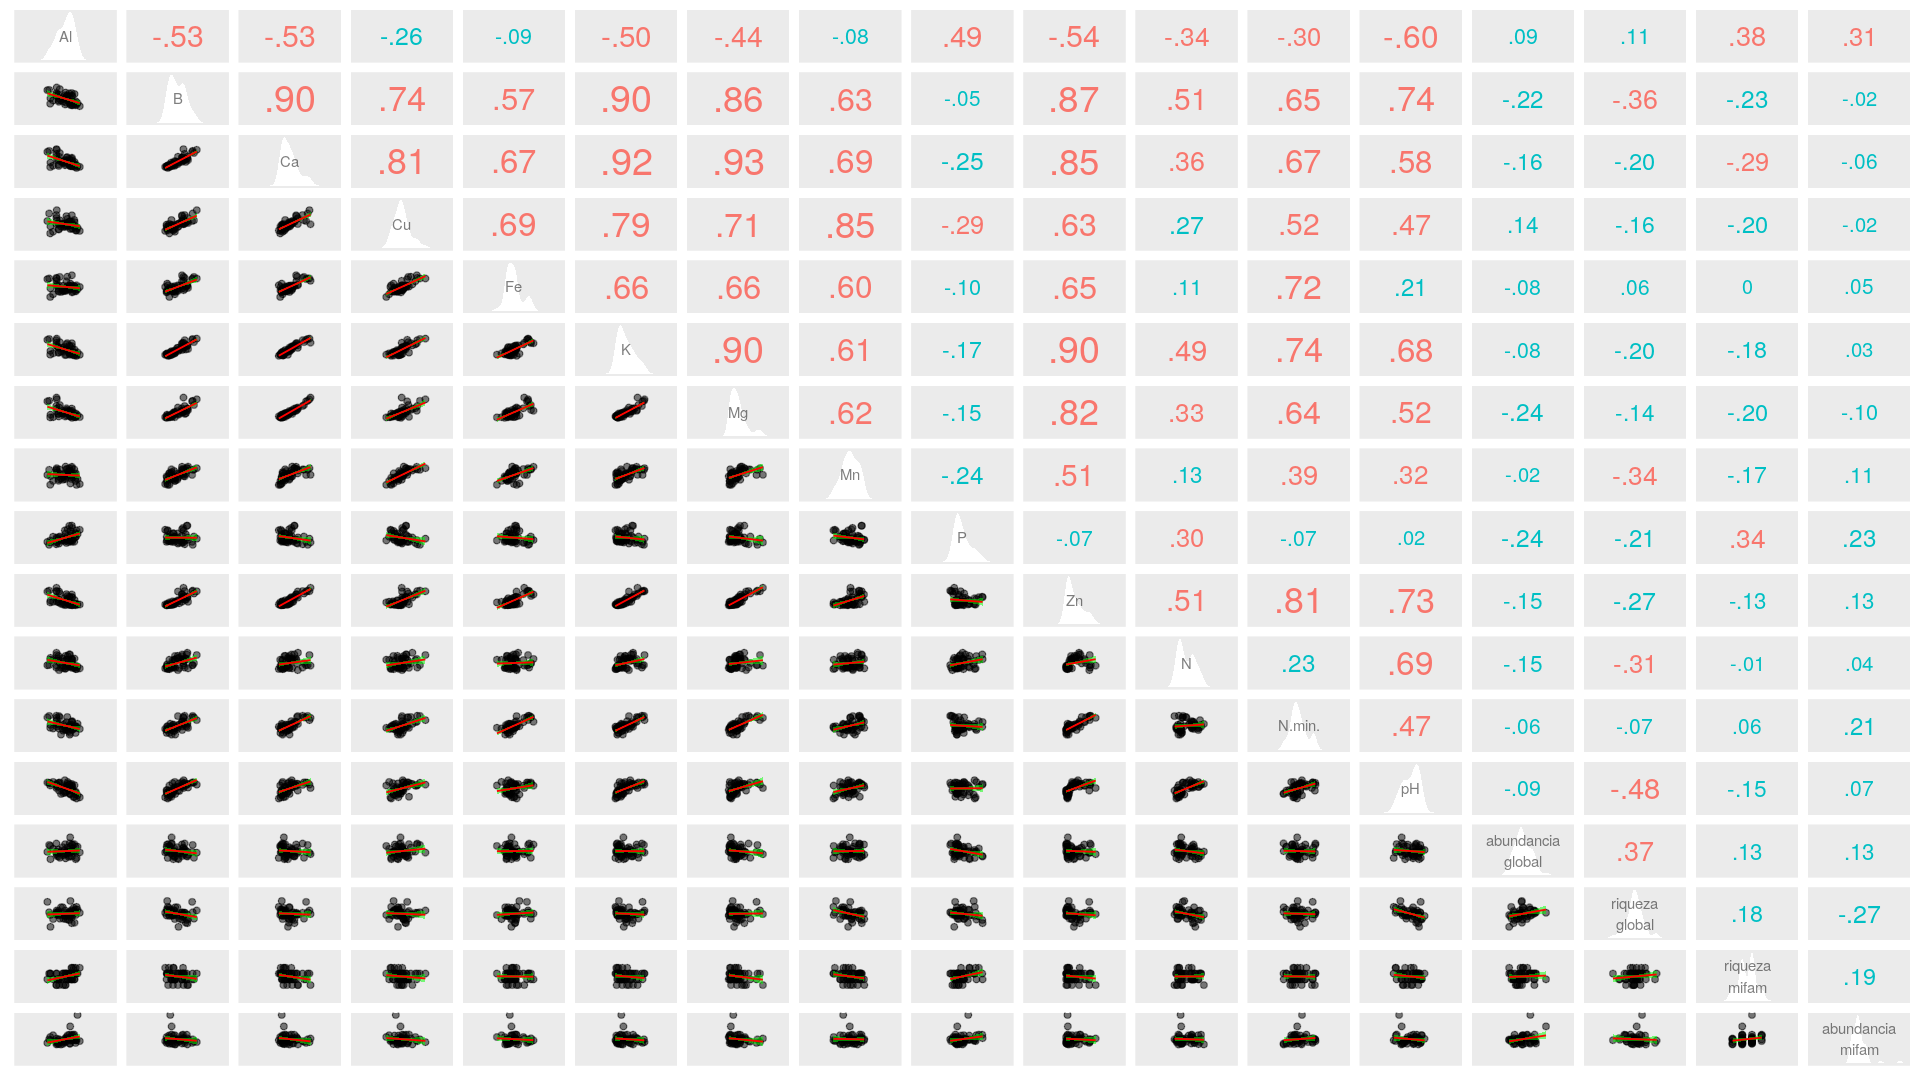
\includegraphics{matriz_correlacion_suelo_abun_riq_spearman.png}
\caption{Matriz de correlación, índice de Spearman
\label{fig:matriz_spearman}}
\end{figure}

El método de agrupamiento Ward de varianza mínima en comparación con el
mapa de calor sugiere que las mirtáceas de la parcela permanente de
50-ha de BCI se distribuyen en 4 grupos, de 2, 13, 15 y 20 sitios,
respectivamente (ver mapa \ref{fig:mapa_ward}). Los métodos de
agrupamiento aglomerativos por enlace simple, por enlace completo y por
enlace promedio (grupos de pares no ponderados con media aritmética,
UPGMA por sus siglas en inglés) destacan la singularidad de este grupo
formado por dos sitios (14 y 19), en suma, el muestreo de bootstrap
multiescalar respalda este grupo con un probabilidad de bootstrap (BP)
de 76 \% y probabilidad de valores aproximadamente insesgados (AU) de 99
\%, de que se un grupo real (ver dendrograma
\ref {fig:bootstrap_multiescalar}). No hay patrones consistentes con
alguna variable ambiental o atributo, aunque las mirtáceas tienen claras
preferencias por el conjunto de variables (Al, Fe, Mn, N. min., etc ) y
atributos del terreno (curvatura perfil media, curvatura tangencial
media, elevación media, etc.) (ver correlograma
\ref{fig:ward_con_variables}).

\begin{figure}
\centering
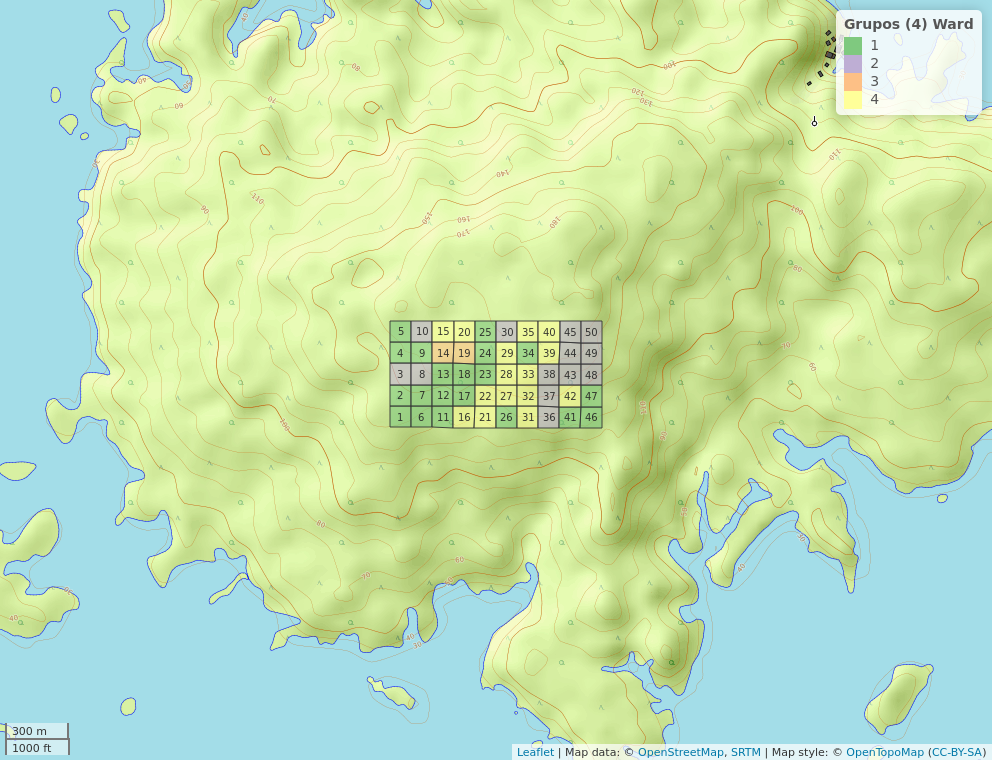
\includegraphics[width=0.50000\textwidth]{mapa_ward_k4.png}
\caption{Agrupamiento por el método Ward de varianza mínima de las
mirtáceas \label{fig:mapa_ward}}
\end{figure}

\begin{figure}
\centering
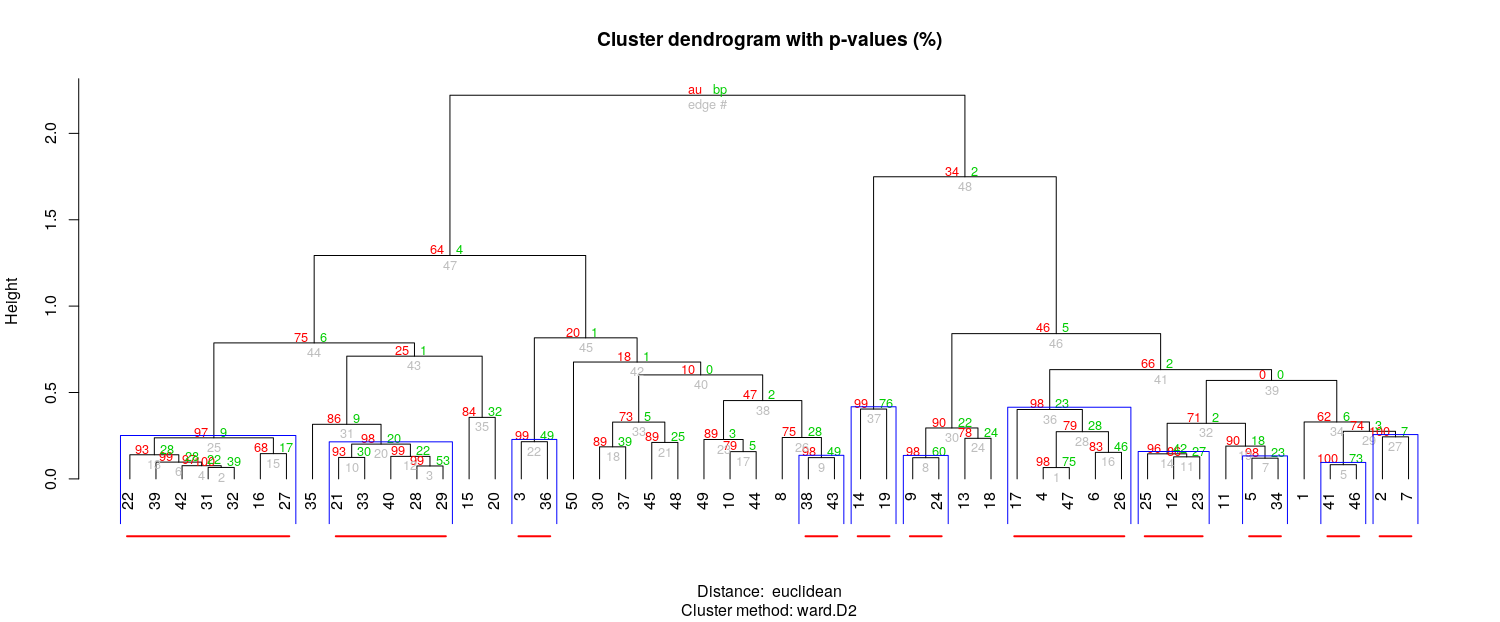
\includegraphics{bootstrap_Ward.png}
\caption{Dendrograma, agrupamiento Ward con los porcentajes del
remuestreo de bootstrap multiescalar \label{fig:bootstrap_multiescalar}}
\end{figure}

\begin{figure}
\centering
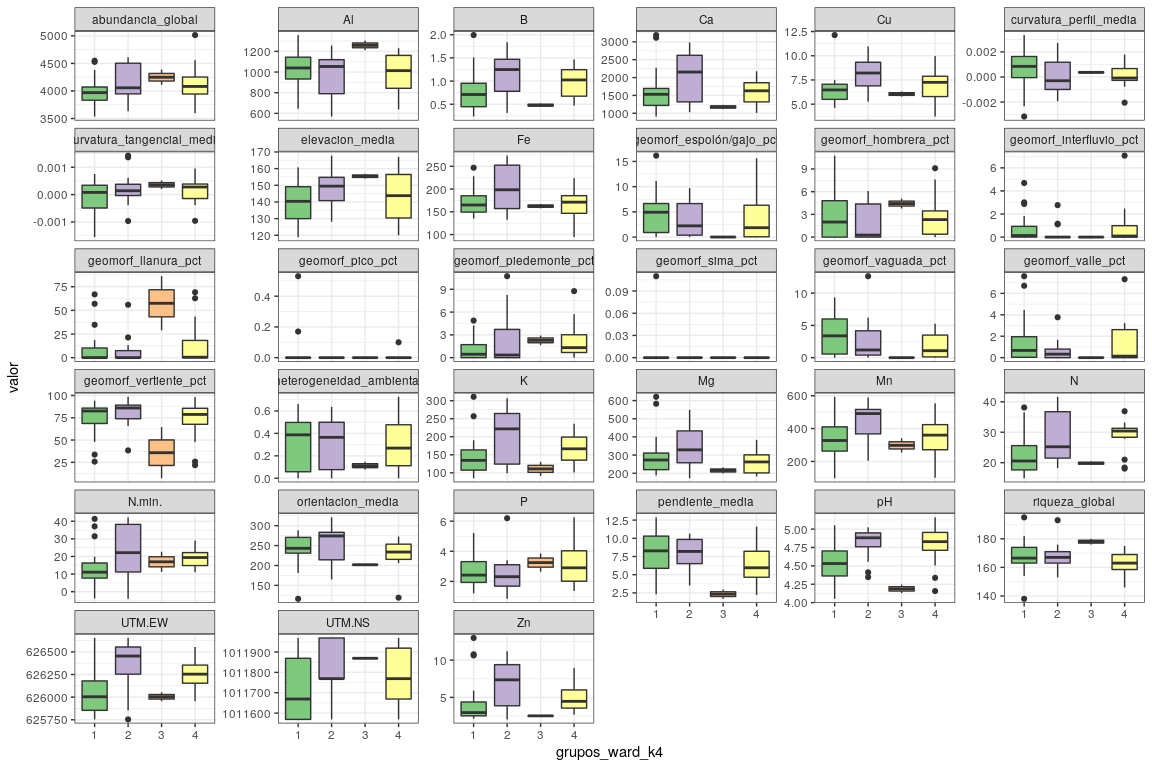
\includegraphics{correlograma_wardyvariablesambientales.png}
\caption{Correlograma grupos Ward con variables ambientales y atributos
\label{fig:ward_con_variables}}
\end{figure}

Para este agrupamiento, el análisis de especies indicadoras mediante
IndVal para una significancia menor de 0.005, propuso como especie
asociada como indicadora del grupo 3 a \emph{Chamguava schippii}, para
el conjunto de grupos 1+2 \emph{Eugenia coloradoensis} y para el
conjunto de grupos 3+4 \emph{Eugenia oerstediana}; y el análisis de
especies con preferencia por hábitat mediante el coeficiente de
correlación biserial puntual para una significancia menor de 0.005,
sugirió que \emph{Eugenia coloradoensis} tiene preferencia por el grupo
2, \emph{Chamguava schippii} por el grupo 3 y \emph{Eugenia oerstediana}
por el grupo 4.

Según los análisis de estimación de riqueza (Homogeneous model,
Homogeneous, los Chao y los Jacknife), la completitud de muestra se
alcanzó al 100\% para las mirtáceas de este ámbito geográfico por lo que
no sería necesario aumentar el esfuerzo de muestreo ya que no se espera
encontrar otras especies en BCI. La diversidad alpha para los grupos
Ward, los cuatro presentaban la riqueza máxima (7 especies) con
diferentes abundancias (1882, 1205, 553 y 1939, respectivamente). Para
los grupos Ward, la riqueza máxima fue estimada y observada, por lo que
también se alcanzó la completitud de muestra al 100\% y al 98\% para el
grupo 3 (grupo con la menor abundancia), y no será necesario aumentar
los esfuerzos de muestreo.

Con relación a la diversidad alpha, la riqueza (N0), E2 y N2 de Hill
sugieren que la diversidad de mirtáceas presenta una correlación
positiva importante con Al, P, Ca y Fe, en suma la equidad de Pielou
(J), los ratios de Hill (E1 y E2) y N2 infieren una correlación positiva
notable con la presencia de la geomorfología de pendiente media.

\emph{Changuava schipii} y \emph{Eugenia oerstediana} son las especies
que hacen contribución a la diversidad beta, éstas están bien
representadas (la primera con gran dominancia) en los sitios 14 y 19
(grupo 3 Ward) que hacen contribución a la diversidad beta, el 14 es uno
de los cinco sitios que poseen la riqueza máxima (los demás sitios son
13, 17, 22 y 40). Este patrón puede estar relacionado con las
preferencias de este grupo.

La prueba I de Moran sugiere que las mirtáceas de esta localización
presentan patrones aglomerados al menos con la vecindad de primer orden
que implica hasta 50 sitios, con excepción de \emph{M. gatunensis} que
muestra un patrón espacial aleatorio. Cabe destacar que para \emph{C.
schipii} existe una autocorrelación espacial en términos positivos
también para los vecinos de segundo orden y en términos negativos del
cuarto al sexto orden e infiero que puede estar asociada a la
distribución Al, P, Fe, bajos valores de Cu, N. min., y la geomorfología
de curvatura perfil media y orientación media ; y para \emph{E.
nesiotica} y \emph{E. oerstediana} una autocorrelacion negativa con
vecinos de tercer a cuarto orden y de cuarto a quinto orden,
respectivamente, es decir, su abundancia disminuye en esas vecindades
cuando aumenta en la de primer orden y viceversa. Los modelos de
distribución de especies (SDM) parecen estar prediciendo bien la
ocurrencia de dichas especies.

\section{Discusión}\label{discusiuxf3n}

\section{Agradecimientos}\label{agradecimientos}

\section{Información de soporte}\label{informaciuxf3n-de-soporte}

\ldots

\section{\texorpdfstring{\emph{Script}
reproducible}{Script reproducible}}\label{script-reproducible}

\ldots

\section*{Referencias}\label{referencias}
\addcontentsline{toc}{section}{Referencias}

\hypertarget{refs}{}
\hypertarget{ref-mapview}{}
Appelhans, T., Detsch, F., Reudenbach, C., \& Woellauer, S. (2019).
\emph{Mapview: Interactive viewing of spatial data in r}. Retrieved from
\url{https://CRAN.R-project.org/package=mapview}

\hypertarget{ref-jose_ramon_martinez_batlle_2020_4402362}{}
Batlle, J. R. M. (2020). biogeografia-master/scripts-de-analisis-BCI:
Long coding sessions (Version v0.0.0.9000).
\url{https://doi.org/10.5281/zenodo.4402362}

\hypertarget{ref-leaflet}{}
Cheng, J., Karambelkar, B., \& Xie, Y. (2018). \emph{Leaflet: Create
interactive web maps with the javascript 'leaflet' library}. Retrieved
from \url{https://CRAN.R-project.org/package=leaflet}

\hypertarget{ref-webcenso}{}
Hubbell, S., Condit, R., \& Foster, R. (2021). Forest Census Plot on
Barro Colorado Island. Retrieved May 5, 2021, from
\url{http://ctfs.si.edu/webatlas/datasets/bci/}

\hypertarget{ref-vegan}{}
Oksanen, J., Blanchet, F. G., Friendly, M., Kindt, R., Legendre, P.,
McGlinn, D., \ldots{} Wagner, H. (2019). \emph{Vegan: Community ecology
package}. Retrieved from \url{https://CRAN.R-project.org/package=vegan}

\hypertarget{ref-sf}{}
Pebesma, E. (2018). Simple Features for R: Standardized Support for
Spatial Vector Data. \emph{The R Journal}, \emph{10}(1), 439--446.
\url{https://doi.org/10.32614/RJ-2018-009}

\hypertarget{ref-perez2005metodologia}{}
Pérez, R., Aguilar, S., Condit, R., Foster, R., Hubbell, S., \& Lao, S.
(2005). Metodologia empleada en los censos de la parcela de 50 hectareas
de la isla de barro colorado, panamá. \emph{Centro de Ciencias
Forestales Del Tropico (CTFS) Y Instituto Smithsonian de Investigaciones
Tropicales (STRI)}, 1--24.

\hypertarget{ref-citadeR}{}
R Core Team. (2019). \emph{R: A language and environment for statistical
computing}. Retrieved from \url{https://www.R-project.org/}

\hypertarget{ref-tidyverse}{}
Wickham, H. (2017). \emph{Tidyverse: Easily install and load the
'tidyverse'}. Retrieved from
\url{https://CRAN.R-project.org/package=tidyverse}

\hypertarget{ref-wilson2010myrtaceae}{}
Wilson, P. G. (2010). Myrtaceae. In \emph{Flowering plants. eudicots}
(pp. 212--271). Springer.




\newpage
\singlespacing 
\end{document}
